\chapter{IMPLEMENTATION DETAILS AND SOFTWARE ARCHITECTURE}

\section{DEVELOPMENT ENVIRONMENT AND DEPENDENCY STACK}
The reference implementation of the HPQV protocol is engineered as a clean, modular Python 3.11 package comprising approximately 1,100 lines of core protocol code (excluding automated test suites and evaluation drivers). The software stack leverages high-performance C libraries accessed via Foreign Function Interfaces (FFI) and ctypes:

\begin{table}[htbp]
    \centering
    \caption{HPQV Implementation Technology Stack and Dependencies.}
    \label{tab:tech_stack}
    \begin{tabularx}{\textwidth}{>{\raggedright\arraybackslash}p{2.6cm} >{\raggedright\arraybackslash}p{3.2cm} c >{\raggedright\arraybackslash}X}
        \toprule
        \textbf{Component} & \textbf{Library / Package} & \textbf{Version} & \textbf{Architectural Responsibility} \\
        \midrule
        Runtime & CPython & 3.11.9 & Pinned execution environment managed via \texttt{uv}. \\
        Post-Quantum Crypto & \texttt{liboqs} / \texttt{liboqs-python} & 0.10.0 & C-based primitives for ML-KEM-768 and ML-DSA-65. \\
        Symmetric Crypto & \texttt{cryptography} (PyCA) & 42.0.5 & ChaCha20-Poly1305 AEAD and HKDF-SHA256 expansion. \\
        Audio Codec & \texttt{libopus} / \texttt{opuslib} & 3.0.1 & Low-latency speech compression and in-band FEC. \\
        Audio I/O & \texttt{sounddevice} / PortAudio & 0.4.6 & Full-duplex microphone capture and speaker rendering. \\
        User Interface & \texttt{tkinter} & Stdlib & Desktop graphical interface with live loss slider. \\
        Testing Harness & \texttt{pytest} & 8.1.1 & Automated unit, integration, and security verification. \\
        \bottomrule
    \end{tabularx}
\end{table}

\section{RUNTIME ANOMALIES AND SYSTEM WORKAROUNDS}
During the engineering of the prototype, several non-trivial cross-platform runtime bugs were identified and resolved:

\subsection{Opuslib In-Band FEC Binding Defect}
In \texttt{opuslib 3.0.1}, the Python property setter \texttt{inband\_fec} contains an upstream ctypes binding defect: the wrapper function fails to forward the integer boolean argument to the underlying C function, rendering \texttt{encoder.inband\_fec = True} a silent no-op. To ensure that Forward Error Correction (LBRR) is properly activated in the C runtime, \texttt{hpqv.audio} bypasses the property setter and invokes the native encoder control routine directly:
\begin{lstlisting}[language=Python]
# Workaround for upstream ctypes binding defect in opuslib 3.0.1
opuslib.api.encoder.encoder_ctl(
    self.enc.encoder_state, 
    opuslib.api.ctl.set_inband_fec, 
    1
)
self.enc.packet_loss_perc = 10
\end{lstlisting}

\subsection{Dynamic Linker Resolution under macOS SIP}
On macOS systems, System Integrity Protection (SIP) scrubs dynamic library search paths for spawned subprocesses. Consequently, \texttt{ctypes.util.find\_library('opus')} returns \texttt{None}, preventing \texttt{opuslib} from discovering Homebrew-installed shared libraries in \texttt{/opt/homebrew/lib}. This was resolved by injecting the fallback linker variable \texttt{DYLD\_FALLBACK\_LIBRARY\_PATH=/opt/homebrew/lib} across test configurations and CLI runners.

\subsection{Cross-Platform Socket Configuration for DF Bit}
Setting the IP Don't-Fragment bit requires distinct low-level operating system socket options across UNIX and Windows kernels. HPQV encapsulates this in \texttt{hpqv.udp}:
\begin{lstlisting}[language=Python]
import socket, sys

def make_udp_socket():
    sock = socket.socket(socket.AF_INET, socket.SOCK_DGRAM)
    if sys.platform.startswith("linux"):
        # IP_MTU_DISCOVER with IP_PMTUDISC_DO (sets DF bit)
        sock.setsockopt(socket.IPPROTO_IP, 10, 2)
    elif sys.platform == "win32":
        # IP_DONTFRAGMENT flag
        sock.setsockopt(socket.IPPROTO_IP, 14, 1)
    return sock
\end{lstlisting}

\section{CORE SYSTEM MODULE BREAKDOWN}
The codebase is partitioned into eight focused modules within \texttt{src/hpqv/}:

\begin{figure}[htbp]
    \centering
    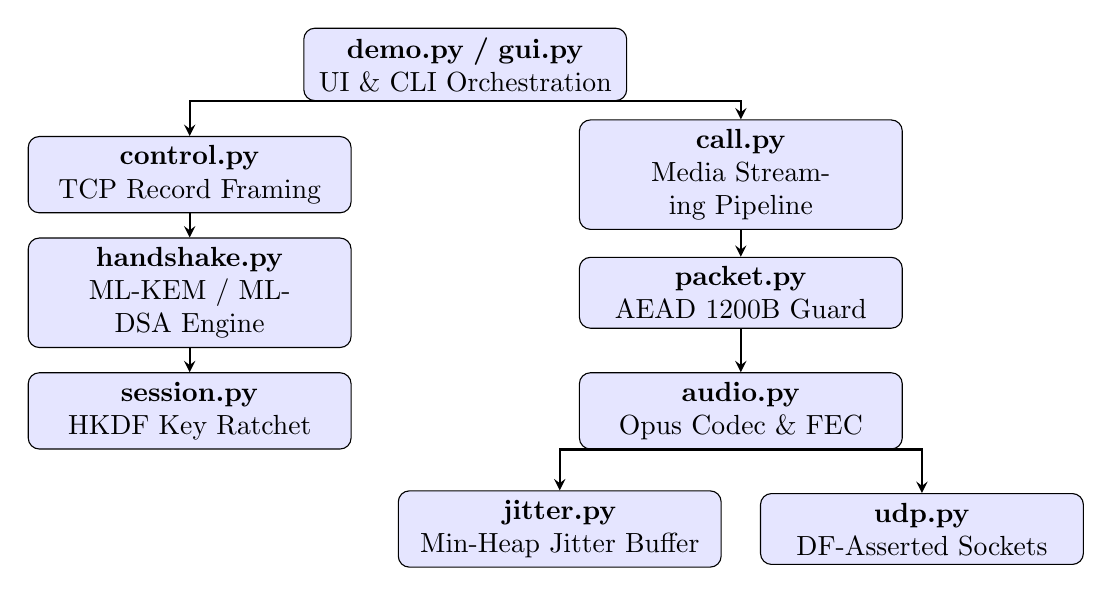
\begin{tikzpicture}[
        every node/.style={align=center},
        mod/.style={rectangle, draw, fill=blue!10, text width=11em, align=center, rounded corners, minimum height=2.4em},
        conn/.style={thick, ->, >=stealth}
    ]
        \node [mod] (demo) at (0, 4.0) {\textbf{demo.py / gui.py}\\UI \& CLI Orchestration};
        
        \node [mod] (ctrl) at (-3.5, 2.6) {\textbf{control.py}\\TCP Record Framing};
        \node [mod] (call) at (3.5, 2.6) {\textbf{call.py}\\Media Streaming Pipeline};
        
        \node [mod] (hs) at (-3.5, 1.1) {\textbf{handshake.py}\\ML-KEM / ML-DSA Engine};
        \node [mod] (sess) at (-3.5, -0.4) {\textbf{session.py}\\HKDF Key Ratchet};
        
        \node [mod] (pkt) at (3.5, 1.1) {\textbf{packet.py}\\AEAD 1200B Guard};
        \node [mod] (aud) at (3.5, -0.4) {\textbf{audio.py}\\Opus Codec \& FEC};
        \node [mod] (jit) at (1.2, -1.9) {\textbf{jitter.py}\\Min-Heap Jitter Buffer};
        \node [mod] (udp) at (5.8, -1.9) {\textbf{udp.py}\\DF-Asserted Sockets};

        \draw [conn] (demo.south) -| (ctrl.north);
        \draw [conn] (demo.south) -| (call.north);
        \draw [conn] (ctrl) -- (hs);
        \draw [conn] (hs) -- (sess);
        \draw [conn] (call) -- (pkt);
        \draw [conn] (pkt) -- (aud);
        \draw [conn] (aud.south) -| (jit.north);
        \draw [conn] (aud.south) -| (udp.north);
    \end{tikzpicture}
    \caption{Module Interaction and Dependency Architecture of HPQV.}
    \label{fig:module_architecture}
\end{figure}

\subsection{Cryptographic Handshake Engine (\texttt{handshake.py})}
Implements the core post-quantum primitives using \texttt{liboqs-python}:
\begin{itemize}
    \item \texttt{make\_identity()}: Generates a long-term ML-DSA-65 identity keypair $(\text{pk}_{\text{DSA}}, \text{sk}_{\text{DSA}})$.
    \item \texttt{build\_hello(sig\_pub, sig\_secret)}: Generates an ephemeral ML-KEM-768 keypair, signs $\text{pk}_{\text{KEM}} \parallel \text{pk}_{\text{DSA}}$, and packs the 6,445-byte \texttt{HELLO} record.
    \item \texttt{accept\_hello(hello, trusted\_sig\_pub, sig\_secret)}: Parses \texttt{HELLO}, asserts pinned identity matching, verifies the caller's signature, encapsulates a 256-bit shared secret, signs $\text{pk}_{\text{KEM}} \parallel \text{ct}_{\text{KEM}}$, derives keys via HKDF, and returns the 4,397-byte \texttt{ACCEPT} record.
    \item \texttt{finish(accept, kem, kem\_pub, trusted\_sig\_pub)}: Verifies the responder's signature against the pinned identity, decapsulates the shared secret, and derives symmetric session keys.
\end{itemize}

\subsection{Control Framing Driver (\texttt{control.py})}
Provides reliable length-prefixed I/O over TCP sockets:
\begin{lstlisting}[language=Python]
import struct

def send_record(sock, payload: bytes) -> None:
    sock.sendall(struct.pack(">I", len(payload)) + payload)

def _recvn(sock, n: int) -> bytes:
    buf = b""
    while len(buf) < n:
        chunk = sock.recv(n - len(buf))
        if not chunk:
            raise ConnectionError("peer closed")
        buf += chunk
    return buf

def recv_record(sock) -> bytes:
    (length,) = struct.unpack(">I", _recvn(sock, 4))
    return _recvn(sock, length)
\end{lstlisting}

\subsection{Packet Serialization and AEAD Sealing (\texttt{packet.py})}
Constructs and validates voice datagrams:
\begin{lstlisting}[language=Python]
import struct
from cryptography.hazmat.primitives.ciphers.aead import ChaCha20Poly1305

MAX_DATAGRAM = 1200
VERSION, TYPE_VOICE = 1, 1

def _header(seq: int, flags: int) -> bytes:
    return struct.pack(">BBQB", VERSION, TYPE_VOICE, seq, flags)

def seal(key, nonce_prefix, seq, opus_frame, flags=0):
    header = _header(seq, flags)
    nonce = nonce_prefix + struct.pack(">Q", seq)
    ct = ChaCha20Poly1305(key).encrypt(nonce, opus_frame, header)
    dg = header + ct
    if len(dg) > MAX_DATAGRAM:
        raise ValueError(f"datagram {len(dg)} > {MAX_DATAGRAM}")
    return dg
\end{lstlisting}

\section{DESKTOP DEMONSTRATION AND GRAPHICAL USER INTERFACE}

\subsection{Command-Line Interface (\texttt{demo.py})}
The system provides a complete CLI interface supporting three primary commands:
\begin{enumerate}
    \item \texttt{keygen --out identity.json}: Generates paired ML-DSA-65 identity keys for caller and listener.
    \item \texttt{listen --port 9000 --identity-file identity.json}: Runs the answering responder daemon.
    \item \texttt{call <IP:port> --identity-file identity.json}: Initiates a secure call to the remote endpoint.
\end{enumerate}
Audio frames can be sourced live from the microphone via \texttt{sounddevice} or read from pre-recorded PCM WAV files with 20 ms frame pacing.

\subsection{Interactive Graphical User Interface (\texttt{gui.py})}
To facilitate live peer evaluations, HPQV includes an interactive Tkinter graphical interface. The GUI features:
\begin{itemize}
    \item \textbf{Asynchronous Threading Architecture:} All socket I/O and cryptographic operations run on dedicated background worker threads. A thread-safe \texttt{queue.Queue} transmits status events to the main thread, polled via \texttt{root.after(200, self.\_poll)} to prevent GUI freezing.
    \item \textbf{Live Audio VU Meters:} Progress bars monitor outbound and inbound RMS audio energy in real time.
    \item \textbf{Dynamic In-Call Packet Loss Slider:} Allows an operator to adjust synthetic packet drop probabilities (from 0\% to 50\%) in real time during an ongoing live call. The audience can directly hear speech degrade and recover as the slider is manipulated, while the dropped packet telemetry counter updates live.
\end{itemize}

\section{AUTOMATED TESTING AND VERIFICATION SUITE}
The implementation is validated by a rigorous test suite comprising 53 automated unit and integration tests executing under \texttt{pytest}.

\begin{table}[htbp]
    \centering
    \caption{Distribution and Verification Targets of the 53-Case Automated Test Suite.}
    \label{tab:test_suite}
    \small
    \begin{tabularx}{\textwidth}{>{\raggedright\arraybackslash}p{4.2cm} c >{\raggedright\arraybackslash}X}
        \toprule
        \textbf{Test Module} & \textbf{Count} & \textbf{Protected Invariants and Behavioral Verification} \\
        \midrule
        \texttt{test\_handshake.py} & 4 & Key agreement derivation, mutual auth, rejection of forged ACCEPT or tampered ciphertext. \\
        \texttt{test\_control.py} & 3 & Framing record round-trip, TCP control state machine, signaling message delivery. \\
        \texttt{test\_session.py} & 2 & Lockstep HKDF key ratcheting, verification of forward secrecy and key modification. \\
        \texttt{test\_packet.py} & 3 & AEAD round-trip, sequence enforcement, strict rejection of datagrams exceeding 1,200 bytes. \\
        \texttt{test\_jitter.py} & 2 & Packet reordering via min-heap, duplicate suppression, late packet drop, clean buffer flush. \\
        \texttt{test\_audio.py} & 1 & Opus 48 kHz / 20 ms encode-decode round-trip fidelity. \\
        \texttt{test\_udp.py} & 1 & Platform-specific socket creation and DF bit assertion. \\
        \texttt{test\_call.py} & 2 & Localhost end-to-end call, verification of directional nonce prefix divergence. \\
        \texttt{test\_loss\_control.py} & 2 & Dynamic loss parameter modification during active audio streaming. \\
        \texttt{eval/test\_mos.py} & 5 & ITU-T G.107 E-model monotonicity, clamping, and continuity at knee boundary. \\
        \texttt{eval/test\_fec\_recovery.py} & 3 & Opus in-band FEC frame recovery and monotonic SNR degradation under loss. \\
        \texttt{eval/test\_handshake\_survival.py} & 3 & Empirical failure of fragmented UDP handshake vs. 100\% survival of hybrid TCP. \\
        \texttt{eval/test\_capture.py} & 2 & Accurate detection of IP fragments in PCAP traces using TShark filters. \\
        \texttt{eval/test\_baselines.py} & 2 & Verification that naive UDP creates 8 fragments while TCP baseline operates cleanly. \\
        \texttt{eval/test\_pqc\_cost.py} & 3 & Calibration of ML-KEM-768 / ML-DSA-65 byte sizes and CPU execution timings. \\
        \texttt{eval/test\_ns3\_smoke.py} & 2 & Compilation and execution integrity of the NS-3 C++ simulation model. \\
        \texttt{Miscellaneous} & 13 & Smoke tests, table renderer sync tests, NetEm teardown cleanup tests. \\
        \midrule
        \textbf{Total Test Cases} & \textbf{53} & \textbf{100\% Pass in Linux Container (38 pass, 15 clean skips on macOS).} \\
        \bottomrule
    \end{tabularx}
\end{table}
